\documentclass{article}
\usepackage{tikz}
\usetikzlibrary{shapes.geometric, positioning, arrows.meta}

% --- Reusable node and arrow styles ---
\tikzset{
  startstop/.style = {
    ellipse, draw, fill=green!15,
    minimum width=2.8cm, minimum height=1cm,
    text centered, font=\small,
  },
  process/.style = {
    rectangle, draw, fill=blue!10,
    minimum width=3.2cm, minimum height=1cm,
    text centered, rounded corners=3pt, font=\small,
  },
  decision/.style = {
    diamond, draw, fill=orange!15, aspect=2.2,
    minimum width=3.2cm, minimum height=1cm,
    text centered, font=\small,
  },
  arrow/.style = {thick, -{Stealth}},
}

\begin{document}

\begin{figure}[h]
  \centering
  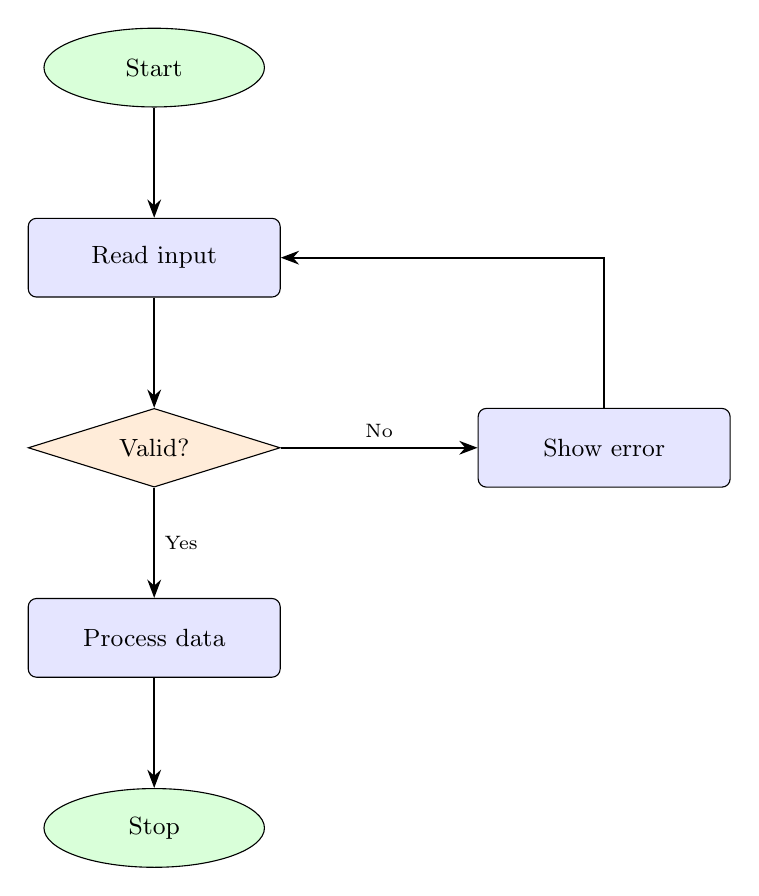
\begin{tikzpicture}[node distance=1.4cm]
    % --- Nodes ---
    \node[startstop]             (start)  {Start};
    \node[process, below=of start]  (input)  {Read input};
    \node[decision, below=of input] (check)  {Valid?};
    \node[process, below=of check]  (proc)   {Process data};
    \node[process, right=2.5cm of check] (error)  {Show error};
    \node[startstop, below=of proc]  (stop)   {Stop};

    % --- Arrows ---
    \draw[arrow] (start) -- (input);
    \draw[arrow] (input) -- (check);
    \draw[arrow] (check) -- node[right, font=\scriptsize]{Yes} (proc);
    \draw[arrow] (check) -- node[above, font=\scriptsize]{No}  (error);
    \draw[arrow] (proc)  -- (stop);
    % Loop back from error to input
    \draw[arrow] (error.north) |- (input.east);
  \end{tikzpicture}
  \caption{Basic flowchart template.}
  \label{fig:flowchart}
\end{figure}

\end{document}
